\documentclass{article}
\usepackage[utf8]{inputenc}
\usepackage{blindtext}
\usepackage[a4paper, total={6in, 10in}]{geometry}
\usepackage{tikz}
\usepackage{amsmath,amssymb}
\usepackage{mathptmx}
\usetikzlibrary{shapes.geometric}
\usepackage[nomessages]{fp}% http://ctan.org/pkg/fp
\definecolor{B}{HTML}{2E79B2}
\definecolor{W}{HTML}{FF0000}

\usepackage[utf8]{inputenc}

\title{GROUP 1}
\author{Project 1}

\begin{document}
\begin{titlepage}
    \begin{center}
        {\fontsize{70}{70}\selectfont MAT 311}
        
        \vspace{1cm}
        \Huge
        \textbf{Group and Ring}
        
        \vspace{0.5cm}
        \LARGE
        Symmetric Group
        
        \vspace{0.5cm}
        {\fontsize{50}{50}\selectfont Group 1}
        \vspace{0.6cm}        
            
        A project providing solution to  different problems on \\ Symmetric Group.
        \vspace{0.8cm}
            
        \includegraphics[width=0.4\textwidth]{UI logo.png}

        \vspace{1.0cm}
        
        \Large{
         Mathematics (BSc. and B.Ed)\\
        University of Ibadan\\
        Nigeria.\\
        18/09/2023}
            
    \end{center}
\end{titlepage}
\tableofcontents
\begin{center}
\LARGE
\begin{tabular} { |p {1 cm}| p {5 cm} | p {2 cm} | p {5 cm} | p{2.2cm}|}

    \hline
    \multicolumn{5} { | c | }{\LARGE{Contributors}}\\
    \hline
    Sn & Names & Matric & Skill &Signature\\
    \hline
1& Oladejo abdullahi Titlayo & 221382 & maths and webdev Tutor&\\
\hline
 2& Ladoja Abimifoluwa Jemimah & 222667 & copy writing&\\
 \hline
3 & Oladapo Testimony Emmanuel & 222678& NFA&\\
  \hline
 4 & Akinsola, Qudus Oladimeji & 221375 & Graphics Design&\\
\hline
 5&OLUWADARA ADEOLUWA & 222691 & Product Management&\\
  \hline
  4&BLESSING ADEBAYO & 222634& Graphic Design&\\
  \hline
  7&Joshua Ebenezer Dayo & 222665& Graphic Design&\\
  \hline
  8&Olanrewaju Bunmi Emmanuel &222681& Laptop Repair Specialist / content Creator&\\
  \hline
  9 & Falola Micheal Oluwatobi & 223769 &  web Design&\\
 \hline
 10&Oladipupo Joy Oluwatomisin & 230179 & entrepreneur&\\
  \hline
11& Olatunde Victor Olubiyi & 222686 &  NFA&\\
\hline
12& Salawu Peter Sunday & 213922  &  Electrician&\\
    \hline
    
 \end{tabular}
 \end{center}
 \vspace{7.0cm}

\newcommand{\drawGraph}[1]{
\draw [color=black](-3,0) -- (3,0);
\draw [color=black](0,-2) -- (0,3); 
}
\newcommand{\ArrowName}[1]{
\begin{tikzpicture}
    \draw [color=white](0,-3) -- (0,3);
    \draw [color=white](-2,0) -- (2,0);
    \draw[ultra thick, ->](-1,0) -- (1,0);
    \node at (0,0.3) {$#1$};
\end{tikzpicture}
}

\newcommand{\labelForthree}[3]{
\tikzstyle{every node}=[draw,shape=circle];
%\node (v0) at (0:0) {$v_0$};
\node[top color=white] (v1) at (0:1.3){$#1$} ;
\node[top color=white] (v2) at (90:2) {$#2$};
\node[top color=white] (v3) at (2*90:1.2) {$#3$};
}

\newcommand{\drawTriangle}[3]{
\begin{tikzpicture}
    \drawGraph{3}
    \node[regular polygon,
    draw,minimum size=2cm,
    right color=white,left color=white,
    regular polygon sides = 3] (p) at (0,0.5){};
   \labelForthree{#1}{#2}{#3}
\end{tikzpicture}
}

\newcommand{\drawTrianglel}[7]{
\begin{tikzpicture}
    \drawGraph{3}
    \node[regular polygon,
    draw,minimum size=2cm,
    right color=white,left color=white,
    regular polygon sides = 3] (p) at (0,0.5){};
    \draw [dashed,color=black](#4,#5) -- (#6,#7);
   \labelForthree{#1}{#2}{#3}
\end{tikzpicture}
}

\section{\Large{PROJECT 1}}

\Large{Questions}
\begin{enumerate}
    \item construct Dihedral group $D_3$ and $D_5$
    \item Give two-dimensional representation of $D_3$ and $D_5$
    \item let us have your creative pattern with polygon
    \item let us have  creative pattern with symmetric from nature
\end{enumerate}

Solutions
\subsection{DIHEDRAL GROUP OF $D_3$ and $D_5$}
\Large{Dihedral group of  $D_3$}

$D_3$ is a set of symmetries of equilateral triangle  equipped with composition.
i.e $D_3=$\{ $R_0,R_1,R_2,F_0,F_1,F_2$\}

\begin{enumerate}

\item{Rotation to angle $0^0$ anticlockwise ($R_0$)}

\drawTriangle{v_1}{v_2}{v_3}
\ArrowName{R_0}
\drawTriangle{v_1}{v_2}{v_3}


\item{Rotation to angle $120^0$ anticlockwise ($R_1$)}

\drawTriangle{v_1}{v_2}{v_3}
\ArrowName{R_1}
\drawTriangle{v_3}{v_1}{v_2}
\vspace{7cm}
\item{Rotation to angle $240^0$ anticlockwise ($R_2$)}

\drawTriangle{v_1}{v_2}{v_3}
\ArrowName{R_2}
\drawTriangle{v_2}{v_3}{v_1}

\item{Reflection on y-axis ($F_0$)}

\drawTrianglel{v_1}{v_2}{v_3}{0}{-2}{0}{2}
\ArrowName{F_0}
\drawTriangle{v_3}{v_2}{v_1}
\item{Reflection through vertex ($v_3$) ($F_1$)}

\drawTrianglel{v_1}{v_2}{v_3}{-2}{-0.6}{2}{1.7}
\ArrowName{F_1}
\drawTriangle{v_2}{v_1}{v_3}

\item{Reflection through vertex ($v_1$) ($F_2$)}

\drawTrianglel{v_1}{v_2}{v_3}{2}{-0.6}{-2}{1.7}
\ArrowName{F_2}
\drawTriangle{v_1}{v_3}{v_2}
\end{enumerate}
\vspace{4cm}



\newcommand{\labelforthreeii}[3]{
\tikzstyle{every node}=[draw,shape=circle];
%\node (v0) at (0:0) {$v_0$};
\node[top color=white] (v1) at (0:1.3){$#1$} ;
\node[top color=white] (v2) at (90:2) {$#2$};
\node[top color=white] (v3) at (2*90:1.2) {$#3$};
}

\newcommand{\NewOne}[3]{
\begin{tikzpicture}
\draw [color=black](-2,0) -- (2,0);
\draw [color=black](0,-1.7) -- (0,3);
    \node[regular polygon,
    draw,minimum size=2cm,
    right color=white,left color=white,
    regular polygon sides = 3] (p) at (0,0.5){};
   \labelforthreeii{#1}{#2}{#3}
\end{tikzpicture}}
\newcommand{\arrowP}[1]{
\begin{tikzpicture}
    \draw [color=white](0,-3) -- (0,3);
    \draw [color=white](-0.4,0) -- (0.4,0);
    \draw[ultra thick, ->](-0.4,0) -- (0.4,0);
    \node at (0,0.3) {$#1$};
\end{tikzpicture}}

\newcommand{\MidText}[1]{
\begin{tikzpicture}
    \draw [color=white](0,-3) -- (0,3);
    \draw [color=white](-0.4,0) -- (0.4,0);
    \draw[color=white](-0.4,0) -- (0.4,0);
    \node at (0,0.3) {$#1$};
\end{tikzpicture}}

Studying the element we see that we can find two elements that can
be use to generate the group.\\
let $f=F_0, r=R_1,$ and $e=R_0$\\

\begin{enumerate}
    \item  $r^2=R_2$
  
\NewOne{v_1}{v_2}{v_3}
\arrowP{r}
\NewOne{v_3}{v_1}{v_2}
\arrowP{r}
\NewOne{v_2}{v_3}{v_1}
so,  $r^2=R_2$

\item  rf=$F_2$
    
\NewOne{v_1}{v_2}{v_3}
\arrowP{f}
\NewOne{v_3}{v_2}{v_1}
\arrowP{r}
\NewOne{v_1}{v_3}{v_2}
so,  rf=$f_3$

\item  $r^2f=F_1$

\NewOne{v_1}{v_2}{v_3}
\arrowP{f}
\NewOne{v_3}{v_2}{v_1}
\arrowP{r^2}
\NewOne{v_2}{v_1}{v_3}
so, $f_2=r^2f$
\end{enumerate}
Now, we can have our $D_3$ to be:\\
 $D_3=$\{ $e,r,r^2,f,rf,r^2f$\}\\\\
 
The Cayleys table below shows that $D_3$ is a group.\\
\begin{tabular}{| l | l | l | l |l |l |l |}
    
    $\circ$  & e & r& $r^2$& f &rf & $r^2f$ \\ 
    \hline
    e  & e & r& $r^2$& f &rf & $r^2f$ \\
     \hline
    r & r& $r^2$& e & rf & $r^2f$&f \\
    \hline
    $r^2$ &$r^2$ & e& $r$&$r^2f$  &f & $rf$ \\
    \hline
    f &f& $r^2f$& rf& e & $r^2$ & $r$ \\
     \hline
    rf & rf& f & $r^2f$ & r &e& $r^2$ \\
     \hline
    $r^2f$ &$r^2f$&rf &f& $r^2$ & r& e \\
    \hline
    \end{tabular}

\begin{itemize}
    \item Clearly $D_3$ equipped with composition is closed.
    \item the composition of function is known to be associative .
    \item every element n $D_3$ has an inverse 
\item e is the identity element 
\end{itemize}
 
\Large{Therefore $D_3$ is a group.}\\\\


\Large{Dihedral group of $D_5$}

$D_3$ is a set of symmetries of regular pentagon equipped with composition.
i.e $D_5=$\{ $R_0,R_1,R_2,R_3,R_4F_0,F_1,F_2,F_3,F_4$\}


\newcommand{\pentagonDraw}[6]{
\begin{tikzpicture}

\node (p) [draw,rotate=70,minimum size=3cm,regular polygon, regular polygon sides=#1] at (0,-0.4) {};
\tikzstyle{every node}=[draw,shape=circle,color=black];
\node[anchor=1*(360/9)]at(p.corner 1){$V_#2$};
\node[anchor=2*(360/9)]at(p.corner 2){$V_#3$};
\node[anchor=3*(360/9)]at(p.corner 3){$V_#4$};
\node[anchor=4*(360/9)]at(p.corner 4){$V_#5$};
\node[anchor=5*(360/9)]at(p.corner 5){$V_#6$};
\end{tikzpicture}
}

\newcommand{\pentagonDrawNew}[6]{
\begin{tikzpicture}

\node (p) [draw,rotate=70,minimum size=2cm,regular polygon, regular polygon sides=#1] at (0,-0.4) {};
\tikzstyle{every node}=[draw,shape=circle,color=black];
\node[anchor=1*(360/9)]at(p.corner 1){$V_#2$};
\node[anchor=2*(360/9)]at(p.corner 2){$V_#3$};
\node[anchor=3*(360/9)]at(p.corner 3){$V_#4$};
\node[anchor=4*(360/9)]at(p.corner 4){$V_#5$};
\node[anchor=5*(360/9)]at(p.corner 5){$V_#6$};
\end{tikzpicture}
}
\begin{enumerate}
\item{Rotation to angle $0^0$ anticlockwise ($R_0$)}

\pentagonDraw{5}{5}{4}{3}{2}{1}
\ArrowName{R_0}
\pentagonDraw{5}{5}{4}{3}{2}{1}

\item{Rotation to angle $72^0$ anticlockwise ($R_1$)}

\pentagonDraw{5}{5}{4}{3}{2}{1}
\ArrowName{R_1}
\pentagonDraw{5}{1}{5}{4}{3}{2}

\item{Rotation to angle $144^0$ anticlockwise ($R_2$)}

\pentagonDraw{5}{5}{4}{3}{2}{1}
\ArrowName{R_2}
\pentagonDraw{5}{2}{1}{5}{4}{3}

\item{Rotation to angle $216^0$ anticlockwise ($R_3$)}

\pentagonDraw{5}{5}{4}{3}{2}{1}
\ArrowName{R_3}
\pentagonDraw{5}{3}{2}{1}{5}{4}
\item{Rotation to angle $288^0$ anticlockwise ($R_4$)}

\pentagonDraw{5}{5}{4}{3}{2}{1}
\ArrowName{R_4}
\pentagonDraw{5}{4}{3}{2}{1}{5}
\newcommand{\pentagonDrawl}[5]{
\node (p) [draw,rotate=70,minimum size=2.7cm,regular polygon, regular polygon sides=5] at (0,-0.4) {};
\tikzstyle{every node}=[draw,shape=circle,color=black];
\node[anchor=1*(360/9)]at(p.corner 1){$V_#1$};
\node[anchor=2*(360/9)]at(p.corner 2){$V_#2$};
\node[anchor=3*(360/9)]at(p.corner 3){$V_#3$};
\node[anchor=4*(360/9)]at(p.corner 4){$V_#4$};
\node[anchor=5*(360/9)]at(p.corner 5){$V_#5$};
}
\vspace{7cm}

\item{Reflection through y-axis ($F_0$)}

\begin{tikzpicture}
\pentagonDrawl{5}{4}{3}{2}{1}
\draw [dashed,color=black](0,2) -- (0,-2);
\end{tikzpicture}
\ArrowName{F_0}
\pentagonDraw{5}{2}{3}{4}{5}{1}

\item{Reflection along a straight line passing through vertex $v_2$ and midpoint of $v_4$ and $v_5$ ($F_1$)}

\begin{tikzpicture}
\pentagonDrawl{5}{4}{3}{2}{1}
\draw [dashed,color=black](2,0.3) -- (-2,-1.1);
\end{tikzpicture}
\ArrowName{F_1}
\pentagonDraw{5}{4}{5}{1}{2}{3}


\item{Reflection along a straight line passing through vertex $v_3$ and midpoint of $v_1$ and $v_5$  ($F_2$)}

\begin{tikzpicture}
\pentagonDrawl{5}{4}{3}{2}{1}
\draw [dashed,color=black](-1.1,1.2) -- (1.8,-3);
\end{tikzpicture}
\ArrowName{F_2}
\pentagonDraw{5}{1}{2}{3}{4}{5}
\vspace{3cm}
\item{Reflection along a straight line passing through vertex $v_4$ and midpoint of $v_2$ and $v_1$  ($F_3$)}

\begin{tikzpicture}
\pentagonDrawl{5}{4}{3}{2}{1}
\draw [dashed,color=black](1.1,1.2) -- (-1.8,-3);
\end{tikzpicture}
\ArrowName{F_3}
\pentagonDraw{5}{5}{4}{3}{2}{1}

\item{Reflection along a straight line passing through vertex $v_5$ and midpoint of $v_2$ and $v_3$ ($F_4$)}

\begin{tikzpicture}
\pentagonDrawl{5}{4}{3}{2}{1}
\draw [dashed,color=black](-2,0.3) -- (2,-1.1);
\end{tikzpicture}
\ArrowName{F_4}
\pentagonDraw{5}{5}{1}{2}{3}{4}
\end{enumerate}


But we can represent $F_0,F_1,F_2,F_3$ and $F_4$  in terms of f and r.\\
Now, 
let $f_0=f$\\

\vspace{8cm}
\begin{enumerate}
    \item $rf={F_1}$

\MidText{rf=}
\pentagonDrawNew{5}{5}{4}{3}{2}{1}
\arrowP{ f }
\pentagonDrawNew{5}{3}{4}{5}{1}{2}
\arrowP{r}
\pentagonDrawNew{5}{4}{5}{1}{2}{3}
\\\\

\item  $r^2f={F_2}$

\MidText{r^2f=}
\pentagonDrawNew{5}{5}{4}{3}{2}{1}
\arrowP{ f }
\pentagonDrawNew{5}{3}{4}{5}{1}{2}
\arrowP{r^2}
\pentagonDrawNew{5}{5}{1}{2}{3}{4}

\item  $r^3f={F_3}$

\MidText{r^3f=} 
\pentagonDrawNew{5}{5}{4}{3}{2}{1}
\arrowP{f}
\pentagonDrawNew{5}{3}{4}{5}{1}{2}
\arrowP{r^3}
\pentagonDrawNew{5}{1}{2}{3}{4}{5} 


\item $r^4f={F_4}$

\MidText{r^4f=F_4} 
\pentagonDrawNew{5}{5}{4}{3}{2}{1}
\arrowP{f}
\pentagonDrawNew{5}{3}{4}{5}{1}{2}
\arrowP{r^3}
\pentagonDrawNew{5}{3}{4}{5}{1}{2}
\end{enumerate}

Then, we can write $D_5$ as \\
$D_5=\{e,r,r^2,r^3,r^4,f,rf,r^2f,r^3f,r^4f\}$\\

The Cayleys table below shows that $D_5$ is a group.\\
\begin{tabular}{| l | l | l | l |l |l |l |l |l |l |l |}
\hline
$\circ$ & e &$ r $&$ r^2 $&$ r^3 $&$ r^4 $&$ f $&$ rf $&$ r^2f $&$ r^3f $&$ r^4f$ \\
\hline
e &$ e $&$ r $&$ r^2 $&$ r^3 $&$ r^4 $&$ f $&$ rf $&$ r^2f $&$ r^3f $&$ r^4f$ \\
\hline
r &$ r $&$ r^2 $&$ r^3 $&$ r^4 $&$ e $&$ rf $&$ r^2f $&$ r^3f $&$ r^4f $&$ f$ \\
\hline
$r^2$&$ r^2 $&$ r^3 $&$ r^4 $&$ e $&$ r $&$ r^2f $&$ r^3f $&$ r^4f $&$ f $& rf\\
\hline
$r^3$&$ r^3 $&$ r^4 $&$ e $&$ r $&$r^2$&$ r^2f $&$ r^3f $&$ r^4f $&$ f $& rf\\
\hline
$r^4$ &$ r^4 $&$ e $&$ r^2 $&$ r^3  $&$ r^4f $&$ f $& rf& rf &$ r^2f $&$ r^3f$\\
\hline
f &$ f $&$ r^4f $&$ r^3f $&$ r^2f  $&$ rf $&$ e $&$ r^4$&$ r^3 $&$ r^2 $& r\\
\hline
rf& rf &$ f $&$ r^4f $&$ r^3f $&$ r^2f $&$ r  $&$ e $&$ r^4 $&$ r^3 $&$  r^2$ \\
\hline
$r^2f$&$ r^2f $&$ rf $&$ f $&$ r^4f $&$ r^3f $&$ r^2 $&$ r  $&$ e $&$ r^4 $&$ r^3$
\\\hline
$r^3f$& $r^3f $&$r^2f $&$ rf $&$ f $&$ r^4 $&$ r^3 $&$ r^2 $&$ r  $&$ e $&$ r^4$ \\
\hline
$r^4$f& $r^4f$& $r^3f$&$r^2f $&$ rf $&$ f $&$ r^4 $&$ r^3 $&$ r^2 $&r &e\\
\hline
\end{tabular}
\\


\subsection{TWO-DIMENSIONAL REPRESENTATION OF $D_3$ and $D_5$}

\Large{The matrices below give a two-dimensional representation of $D_3$ }\\

For $r_0 \in D_3$ , $\theta = 0$\\

$\phi(r_0) =  $ 
$\begin{pmatrix}
    cos 0 & -sin 0\\
    sin 0 & cos 0
\end{pmatrix}$=$\begin{pmatrix}
    1& 0\\
    0 & 1
\end{pmatrix}$\\

For $r_{120^0} \in D_3$ , $\theta = 120^0$\\

$\phi(r_{120}) =  $ 
$\begin{pmatrix}
    cos 120 & -sin 120\\
    sin 120 & cos 120
\end{pmatrix}$=
$\begin{pmatrix}
   - \frac{1}{2}& -\frac{\sqrt{3}}{2}\\
    \frac{\sqrt{3}}{2} & - \frac{1}{2}
\end{pmatrix}$
\\

For $r_{240^0} \in D_3$ , $\theta = 240^0$\\

$\phi(r_{240}) =  $ 
$\begin{pmatrix}
    cos 240 & -sin 240\\
    sin 240 & cos 240
\end{pmatrix}$=
$\begin{pmatrix}
   - \frac{1}{2}& \frac{\sqrt{3}}{2}\\
    -\frac{\sqrt{3}}{2} & - \frac{1}{2}
\end{pmatrix}$
\\\\

\textbf{Refection parts}\\

$\begin{pmatrix}
    cos \frac{2\pi k}{n} & sin\frac{2\pi k}{n}\\
    sin \frac{2\pi k}{n} & -cos \frac{2\pi k}{n}
\end{pmatrix}$\\\\

When k=0, $\begin{pmatrix}
    1 & 0\\
    0 & 1
\end{pmatrix}$\\\\



When k=1, $\begin{pmatrix}
     - \frac{1}{2} & \frac{\sqrt{3}}{2}\\
    \frac{\sqrt{3}}{2}& \frac{1}{2}
\end{pmatrix}$\\\\

When k=2, 
$\begin{pmatrix}
     - \frac{1}{2} & -\frac{\sqrt{3}}{2}\\
    -\frac{\sqrt{3}}{2}& \frac{1}{2}
\end{pmatrix}$\\\\


\Large{The matrices below give a two-dimensional representation of $D_5$ }\\

\pmb{for $e=r_0 \in D_5, \theta =0^0$}\\
$\phi (r_0) = 
\begin{pmatrix}
cos 0^0 & -sin 0^0\\
sin 0^0 & cos0^0
\end{pmatrix} =
\begin{pmatrix}
1 & 0\\
0 & 1
\end{pmatrix} $\\\\

\pmb{for $r=r_{72^0} \in D_5, \theta =72^0$}\\
$\phi (r_{72^0}) = 
\begin{pmatrix}
cos 72^0 & -sin 72^0\\
sin 72^0 & cos72^0
\end{pmatrix} =
\begin{pmatrix}
\frac{-1+\sqrt{5}}{4} & \frac{-\sqrt(\frac{1}{2}*(5+\sqrt{5}))}{2}\\
\frac{\sqrt(\frac{1}{2}*(5+\sqrt{5}))}{2}& \frac{-1+\sqrt{5}}{4}
\end{pmatrix} $\\\\

\pmb{for $r^3=r_{144^0} \in D_5, \theta =144^0$}\\
$\phi (r_{144^0}) = 
\begin{pmatrix}
cos 144^0 & -sin 144^0\\
sin 144^0 & cos144^0
\end{pmatrix} =
\begin{pmatrix}
\frac{-1-\sqrt{5}}{4} & \frac{-\sqrt(\frac{1}{2}*(5+\sqrt{5}))}{2}\\
\frac{\sqrt(\frac{1}{2}*(5+\sqrt{5}))}{2}& \frac{-1-\sqrt{5}}{4}
\end{pmatrix} $\\\\

\pmb{for $r^3=r_{216^0} \in D_5, \theta =216^0$}\\
$\phi (r_{216^0}) = 
\begin{pmatrix}
cos 216^0 & -sin 216^0\\
sin 216^0 & cos216^0
\end{pmatrix} =
\begin{pmatrix}
\frac{-1-\sqrt{5}}{4} & \frac{\sqrt(\frac{1}{2}*(5+\sqrt{5}))}{2}\\
-\frac{\sqrt(\frac{1}{2}*(5+\sqrt{5}))}{2}& \frac{-1-\sqrt{5}}{4}
\end{pmatrix} $\\\\

\pmb{for $r^4=r_{288^0} \in D_5, \theta =288^0$}\\
$\phi (r_{288^0}) = 
\begin{pmatrix}
cos 288^0 & -sin 288^0\\
sin 288^0 & cos288^0
\end{pmatrix} =
\begin{pmatrix}
\frac{-1+\sqrt{5}}{4} & \frac{\sqrt(\frac{1}{2}*(5+\sqrt{5}))}{2}\\
-\frac{\sqrt(\frac{1}{2}*(5+\sqrt{5}))}{2}& \frac{-1+\sqrt{5}}{4}
\end{pmatrix} $\\\\



\pmb{Reflection}\\
Using the genera formula;\\

$\begin{pmatrix}
cos \frac{2 \pi k}{n} & -sin \frac{2 \pi k}{n}\\
sin \frac{2 \pi k}{n} & cos\frac{2 \pi k}{n}
\end{pmatrix}$
where, n=5, k=0,1,2,3,4\\\\

when k=0,\\\\
$\begin{pmatrix}
1 & 0\\
0 & 1
\end{pmatrix}$\\

when k=1\\\\
$\begin{pmatrix}
\frac{-1+\sqrt{5}}{4} & \frac{\sqrt[]{\frac{1}{2}*(5+\sqrt{5})}}{2}\\\\
\frac{\sqrt{\frac{1}{2}*(5+\sqrt{5})}}{2}& \frac{1-\sqrt{5}}{4}
\end{pmatrix}$ \\


when k=2\\\\
$\begin{pmatrix}
\frac{-1-\sqrt{5}}{4} & \frac{\sqrt{\frac{1}{2}*(5-\sqrt{5})}}{2}\\\\
\frac{\sqrt{\frac{1}{2}*(5-\sqrt{5})}}{2}& \frac{1+\sqrt{5}}{4}
\end{pmatrix}$ \\

when k=3\\\\
$\begin{pmatrix}
\frac{-1-\sqrt{5}}{4} & -\frac{\sqrt{\frac{1}{2}*(5-\sqrt{5})}}{2}\\\\
-\frac{\sqrt{\frac{1}{2}*(5-\sqrt{5})}}{2}& \frac{1+\sqrt{5}}{4}
\end{pmatrix}$ \\\\

when k=4\\\\
$\begin{pmatrix}
\frac{-1+\sqrt{5}}{4} & -\frac{\sqrt(\frac{1}{2}*(5-\sqrt{5}))}{2}\\
-\frac{\sqrt{\frac{1}{2}*(5+\sqrt{5})}}{2}& \frac{1-\sqrt{5}}{4}
\end{pmatrix}$ 
\\\\\\


\pmb{for $e=r_0 \in D_5, \theta =0^0$}\\
$\phi (r_0) = 
\begin{pmatrix}
cos 0^0 & -sin 0^0\\
sin 0^0 & cos0^0
\end{pmatrix} =
\begin{pmatrix}
1 & 0\\
0 & 1
\end{pmatrix} $\\\\

\pmb{for $r=r_{72^0} \in D_5, \theta =72^0$}\\
$\phi (r_{72^0}) = 
\begin{pmatrix}
cos 72^0 & -sin 72^0\\
sin 72^0 & cos72^0
\end{pmatrix} =
\begin{pmatrix}
\frac{-1+\sqrt{5}}{4} & \frac{-\sqrt{\frac{1}{2}*(5+\sqrt{5})}}{2}\\
\frac{\sqrt{\frac{1}{2}*(5+\sqrt{5})}}{2}& \frac{-1+\sqrt{5}}{4}
\end{pmatrix} $\\\\

\pmb{for $r^3=r_{144^0} \in D_5, \theta =144^0$}\\
$\phi (r_{144^0}) = 
\begin{pmatrix}
cos 144^0 & -sin 144^0\\
sin 144^0 & cos144^0
\end{pmatrix} =
\begin{pmatrix}
\frac{-1-\sqrt{5}}{4} & \frac{-\sqrt{\frac{1}{2}*(5+\sqrt{5})}}{2}\\
\frac{\sqrt(\frac{1}{2}*(5+\sqrt{5}))}{2}& \frac{-1-\sqrt{5}}{4}
\end{pmatrix} $\\
\pmb{for $r^3=r_{216^0} \in D_5, \theta =216^0$}\\

$\phi (r_{216^0}) = 
\begin{pmatrix}
cos 216^0 & -sin 216^0\\
sin 216^0 & cos216^0
\end{pmatrix} =
\begin{pmatrix}
\frac{-1-\sqrt{5}}{4} & \frac{\sqrt{\frac{1}{2}*(5+\sqrt{5})}}{2}\\
-\frac{\sqrt{\frac{1}{2}*(5+\sqrt{5})}}{2}& \frac{-1-\sqrt{5}}{4}
\end{pmatrix} $\\\\

\pmb{for $r^4=r_{288^0} \in D_5, \theta =288^0$}\\
$\phi (r_{288^0}) = 
\begin{pmatrix}
cos 288^0 & -sin 288^0\\
sin 288^0 & cos288^0
\end{pmatrix} =
\begin{pmatrix}
\frac{-1+\sqrt{5}}{4} & \frac{\sqrt{\frac{1}{2}*(5+\sqrt{5})}}{2}\\
-\frac{\sqrt{\frac{1}{2}*(5+\sqrt{5})}}{2}& \frac{-1+\sqrt{5}}{4}
\end{pmatrix} $\\\\


$\begin{pmatrix}
cos \frac{2 \pi k}{n} & -sin \frac{2 \pi k}{n}\\
sin \frac{2 \pi k}{n} & cos\frac{2 \pi k}{n}
\end{pmatrix}$
where, n=5, k=0,1,2,3,4\\\\

when k=0,\\
$\begin{pmatrix}
cos 0 & -sin 0\\
sin 0 & cos0
\end{pmatrix}$=
$\begin{pmatrix}
1 & 0\\
0 & 1
\end{pmatrix}$\\

when k=1\\

$\begin{pmatrix}
\frac{-1+\sqrt{5}}{4} & \frac{\sqrt{\frac{1}{2}*(5+\sqrt{5})}}{2}\\
\frac{\sqrt{\frac{1}{2}*(5+\sqrt{5})}}{2}& \frac{1-\sqrt{5}}{4}
\end{pmatrix}$ \\\\

when k=2\\

$\begin{pmatrix}
\frac{-1-\sqrt{5}}{4} & \frac{\sqrt{\frac{1}{2}*(5-\sqrt{5})}}{2}\\
\frac{\sqrt{\frac{1}{2}*(5-\sqrt{5})}}{2}& \frac{1+\sqrt{5}}{4}
\end{pmatrix}$\\\\

when k=3\\

$\begin{pmatrix}
\frac{-1-\sqrt{5}}{4} & -\frac{\sqrt{\frac{1}{2}*(5-\sqrt{5})}}{2}\\\\
-\frac{\sqrt{\frac{1}{2}*(5-\sqrt{5})}}{2}& \frac{1+\sqrt{5}}{4}
\end{pmatrix}$ \\\\

when k=4\\

$\begin{pmatrix}
\frac{-1+\sqrt{5}}{4} & -\frac{\sqrt{\frac{1}{2}*(5-\sqrt{5})}}{2}\\\\
-\frac{\sqrt{\frac{1}{2}*(5+\sqrt{5})}}{2}& \frac{1-\sqrt{5}}{4}
\end{pmatrix}$ 
\vspace{11cm}
\graphicspath{{pictures/}}
\subsection{CREATIVE PATTERN WITH POLYGONS}
\begin{enumerate}
    \item STAR OF UNITED TRIANGLES: this is a pattern expressing the power of unity. A beautiful pattern that can be created on any square or rectangular surface materials. It was named STAR OF UNITED TRIANGLE because two triangles joined together to form this beautiful thing and they covered a the surface by translating the same way. The following steps were taken to arrived at this pattern.

 \textbf{step1}: we start by colored the square surface red. then an regular polygon of three sides(0.7 units) was drawn.
 
 \textbf{step2}: we draw another regular polygon of three sides with the same unit having the same centers coordinate but rotated $180^0$.
 
 \textbf{step 3}: step 1 and 2 was repeated with a unit side less than 0.7.
 
 \textbf{step 4} : A small circle was drawn at the center to beautify it.\\
  \textbf{step 5} : Now with the knowledge of translation in algebra we were able to translate the A the shapes  done from step 1-4 through out the surface by using loop in latex to change the coordinate (x,y). see the pattern below
\begin{figure}[htp]

\includegraphics[width=14.5cm]{starTri.PNG}
\caption{STAR OF UNITED TRIANGLES}
\end{figure}\\


\item STAR OF UNITED PENTAGONS

This pattern was created using method similar to Star of united triangle only that we are using different polygons here we are making use of regular pentagon to draw the pattern. One amazing thing about this pattern is that it can work for all regular polygons and as the sides of the polygon increase we get another kind of star.\\
see the pattern below.
\begin{figure}[htp]

\includegraphics[width=17cm]{starpent.PNG}
\caption{STAR OF UNITED PENTAGONS}
\end{figure}
\end{enumerate}
\vspace{4cm}
\subsection{SYMMETRIC FROM NATURE}
\begin{enumerate}
    \item HONEY BEE HIVES \\
    Honey bee hives are made of six-sided tubes, which are the shapes for optimal honey production because they require less wax and can hold more honey. Some hives develop broods which become dark in color over time because of cocoon tracks and travel stains. Other honey bee hives remain light in color.\\
    See picture of honey bee hives below to see the pattern.\\
    \begin{figure}[htp]
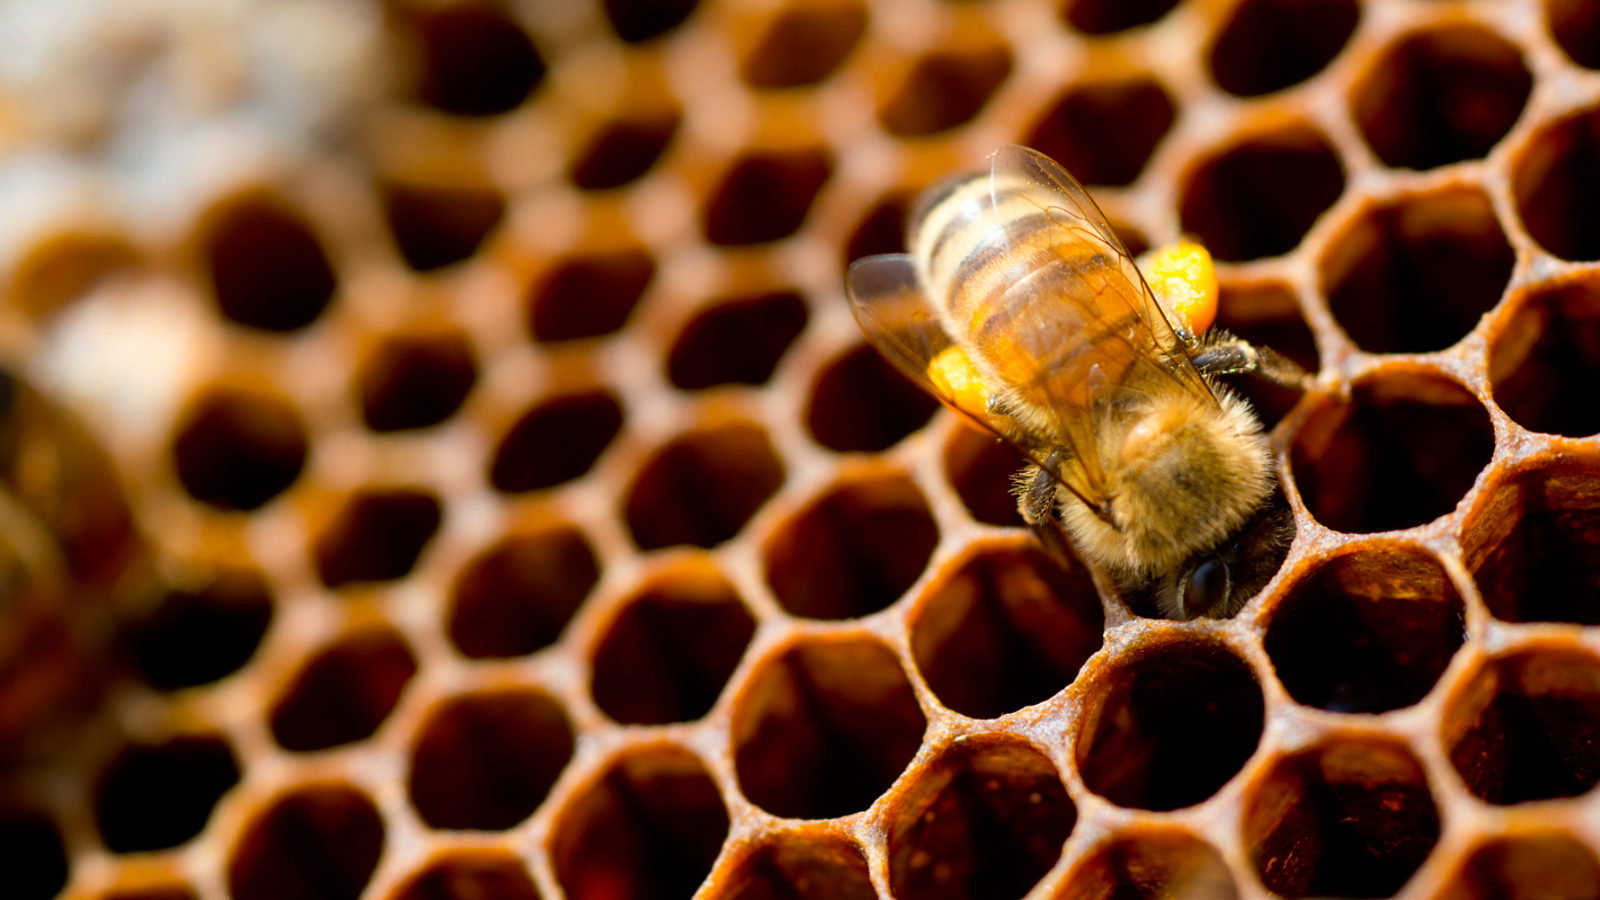
\includegraphics[width=17cm]{Honey.jpg}
\caption{HONEY BEE HIVES}
\end{figure}\\
\item Bisection of Orange \\
When you cut a piece of fruit in half, either side of that piece of fruit will be pretty close to identical. It will have a similar number of seeds on each side, the same lines and shape on each side, and each piece will be a reflection of the other.\\

In fact, sometimes a fruit will also reflect in a circle. Look at the orange in the next page; see how it seems to be made up of several identical pieces that rotate around a center? Symmetry is very similar to cutting that piece of fruit in half.
The Orange has the same rotation as $D_10$
    \begin{figure}[htp]
\includegraphics[width=17cm]{orange.jpg}
\caption{BISECTION OF ORANGE}
\end{figure}\\
\end{enumerate}
\vspace{14cm}
\section{PROJECT 2}\
\textbf{Question}\\

Describe Group of Symmetry of a rectangle\\
\textbf{Solution}\\
\subsection{GROUP OF SYMMETRY OF RECTANGLE}
\newcommand{\Rectang}[4]{
\begin{tikzpicture}
\drawGraph{3} 
\draw (-2,1)[] -| node[pos=0,left]{$v_#1$} 
              node[pos=.5,right]{$v_#2$} 
              (2,-1) -|  node[pos=0,right]{$v_#3$}
  node[pos=.5,left]{$v_#4$} cycle;

\end{tikzpicture}
}

$D_2$ is a set of symmetries of rectangle equipped with composition.
i.e $D_2=$\{ $R_0,R_1,F_0,F_1$\}

\begin{enumerate}
\item{Rotation to angle $0^0$ anticlockwise ($R_0$)}

\Rectang{1}{2}{3}{4}
\ArrowName{R_0}
\Rectang{1}{2}{3}{4}

\item{Rotation to angle $180^0$ anticlockwise ($R_1$)}

\Rectang{1}{2}{3}{4}
\ArrowName{R_1}
\Rectang{3}{4}{1}{2}

\item{Refection through y-axis ($F_0$)}

\Rectang{1}{2}{3}{4}
\ArrowName{F_0}
\Rectang{2}{1}{4}{3}

\item{Refection through x-axis  ($F_1$)}

\Rectang{1}{2}{3}{4}
\ArrowName{F_1}
\Rectang{4}{3}{2}{1}
\end{enumerate}
We can rewrite element in the group for better readability.\\
\newcommand{\rectang}[4]{
\begin{tikzpicture}
\draw [color=black](-2,0) -- (2,0);
\draw [color=black](0,-2) -- (0,2); 
\draw (-1.4,0.7)[] -| node[pos=0,left]{$v_#1$} 
              node[pos=.5,right]{$v_#2$} 
              (1.4,-0.7) -|  node[pos=0,right]{$v_#3$}
  node[pos=.5,left]{$v_#4$} cycle;
\end{tikzpicture}
}


let $R_0=e$,$R_1=r$ and $f=F_0$\\
then, we see that $rf=F_1$ as shown below\\\\
\rectang{1}{2}{3}{4}
\arrowP{r}
\rectang{3}{4}{1}{2}
\arrowP{f}
\rectang{4}{3}{2}{1}


The following table shows Cayley's table below shows that $D_2$ is a group.\\\\

\begin{tabular}{| l | l | l | l |l |}
\hline
$\circ$& e& r & f & rf \\
\hline
e& e& r & f & rf \\
\hline
r& r& e & rf & f\\ 
\hline
f& f& rf& e & r \\
\hline
rf& rf&f &r & e \\
\hline
\end{tabular}
\\\\


\section{PROJECT 3}
\pmb{Questions}
\begin{enumerate}
\item Describe group of symmetry of tetrahedral
\item Describe the symmetry of a cube 
\item Describe square in dimension 4 and 5
\end{enumerate}
\pmb{Solutions}
\subsection{SYMMETRY OF A TETRAHEDRAL}
In order to describe the symmetry of tetrahedral,
 let $v_1, v_2, v_3$ and $ v_4$ be the set of vertices of a tetrahedron, $f_1,f_2,f_3$ and $f_4$ be the set of faces and
 $e_1,e_2,e_3,e_4,e_5$ and $e_6$ as shown
 in figure 4 in the next page.\\

\begin{figure}[htp]
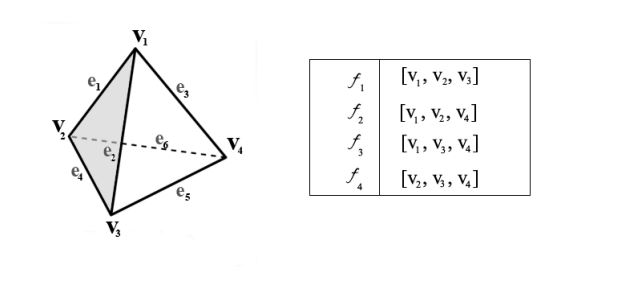
\includegraphics[width=17cm]{prismOrigin.JPG}
\caption{Tetrahedral Faces,Vertex and Edges.}
\end{figure}

\pmb{Rotational Symmetry of a Tetrahedron}\\
Suppose we let the solid be situated with its center at the origin in $\mathcal{R}
_3$. There are 12 rotational symmetry which can be divided in to three categories

\begin{enumerate}
    \item identity ($R_0=e$)
    \item two rotations through $120^0$ and $240^0$ about each of the four axes joining vertices with centres of opposite faces
    \item one rotation through angle $180^0$
about each of 3 axes joining the midpoints of opposites edges.
\end{enumerate}

\newcommand{\Transform}[3]{
  \begin{figure}[htp]
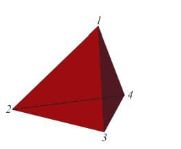
\includegraphics[width=5cm]{prismOrigin1.JPG}
\ArrowName{#1}
\includegraphics[width=5cm]{#2.JPG}
\caption{#3}
\end{figure}
}
\newcommand{\TransformNew}[4]{
  \begin{figure}[htp]
\includegraphics[width=5cm]{#1.JPG}
\ArrowName{#2}
\includegraphics[width=5cm]{#3.JPG}
\caption{#4}
\end{figure}
}


   \Transform{e}{prismOrigin1}{Rotation at Angle zero degree}
   
   \Transform{R_1}{prismOrigin2}{$120^0$ Rotations anticlockwise of axis through vertex 1 ($v_1$) and the centres of opposite faces($f_4)$
}
   
   \Transform{R_2}{prismOrigin3}{$240^0$ Rotations anticlockwise of axis through vertex 1 ($v_1$) and the centres of opposite faces($f_4)$}
   
   \Transform{R_3}{prismOrigin4}{$120^0$ Rotations anticlockwise of axis through vertex 2 ($v_2$) and the centres of opposite faces($f_3)$}
   
   
   \Transform{R_4}{prismOriginv}{$240^0$ Rotations anticlockwise of axis through vertex  ($v_2$) and the centres of opposite faces($f_3)$}

   \Transform{R_5}{prismOriginvi}{$120^0$ Rotations anticlockwise of axis through vertex  ($v_3$) and the centres of opposite faces($f_2)$}
   
   
   \Transform{R_6}{prismOrigin7}{$240^0$ Rotations anticlockwise of axis through vertex  ($v_3$) and the centres of opposite faces($f_2)$}

   \Transform{R_7}{prismOrigin8}{$120^0$ Rotations anticlockwise of axis through vertex  ($v_4$) and the centres of opposite faces($f_1)$}
   
   \Transform{R_8}{prismOrigin9}{$240^0$ Rotations anticlockwise of axis through vertex  ($v_4$) and the centres of opposite faces($f_1)$}

    \TransformNew{prismOrigin14}{R_9}{prismOrigin10}{$180^0$ Rotations anticlockwise of axes joining the midpoints of edge 1 ($e_1$) and  edge 5($e_5)$}

   \TransformNew{prismOrigin1v}{R_{10}}{prismOrigin11}{$180^0$ Rotations anticlockwise of axes joining the midpoints of edge 2 ($e_2$) and edge 6 ($e_6)$}

   \TransformNew{prismOrigin1vi}{R_{11}}{prismOrigin12}{$180^0$  Rotations anticlockwise of axes joining the midpoints of edge 4 ($e_4$) and edge 3 ($e_3)$}
   \vspace{8cm}
   \pmb{Reflectional symmetry of tetrahedral}\\
 There are 12 reflections but 6 unique reflections of a tetrahedron all derived by placing a reflection mirror between the solid from the vertex on top while it rest on one face. These reflections can be illustrated by the
Figure 17 below\\

\begin{figure}[htp]
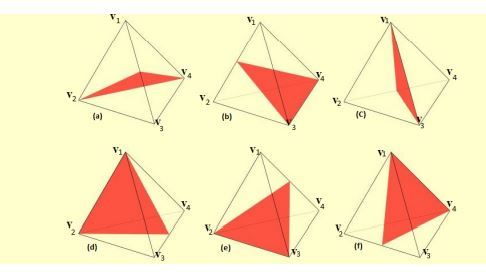
\includegraphics[width=17cm]{prismRef.JPG}
\caption{Reflectiion of Tetrahedral}
\end{figure}\\
In short there are 24 elements in a group of symmetry of a cube
\vspace{9cm}
\subsection{SYMMETRY OF CUBE}
In order to describe the symmetry of a cube,
 let $v_1, v_2, v_3,v_4,v_5,v_6,v_7$ and $ v_8$ be the set of vertices of a cube, $f_1,f_2,f_3,f_4,f_5$ and $f_6$ be the set of faces and $e_1,e_2,e_3,e_4,e_5...,e_{12}$ and $e_6$ as shown
 in figure 4 below.\\

\begin{figure}[htp]
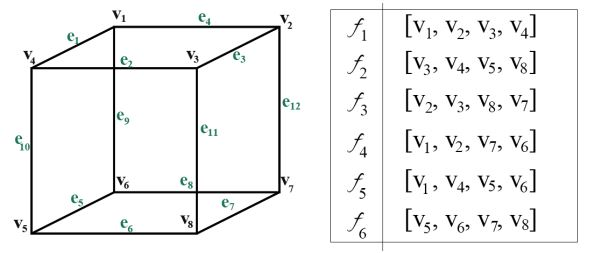
\includegraphics[width=17cm]{cube1.JPG}
\caption{Tetrahedral Faces,Vertex and Edges.}
\end{figure}

\pmb{Rotational Symmetry of a Cube}\\
Suppose we let the solid be situated with its center at the origin in $\mathcal{R}
_3$. There are 12 rotational symmetry which can be divided in to three categories
\begin{enumerate}
    \item The identity ($e)$
    \item  Rotations of an axis through the centres of directly opposite faces about $90^0$, $180^0$ and $270^0$
    \item Rotations of an axis through the midpoints of the 2 diagonally opposite edges about $180^0$
    \item Rotations of an axis through 2 diagonally opposite vertices about $120^0$ and $240^0$
\end{enumerate}

Using the denotations for faces and edges as described tetrahedron we can easily understand it.\\
we can illustrate the above elements using Figure 19 in the next page.\\
\vspace{12cm}

\begin{figure}[htp]
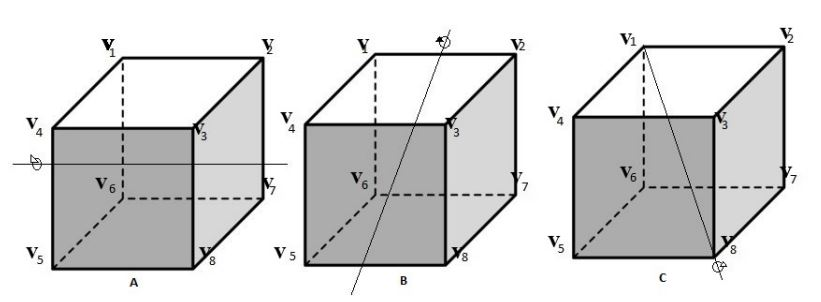
\includegraphics[width=17cm]{cube2.JPG}
\caption{Rotational symmetry axis of a Cube}
\end{figure}
\textbf{Note}: The rotations for  category 2, 3 and 4 are represented by the cubes above respectively.\\

 \textbf{Reflectional Symmetry of a Cube}\\
 
There are 12 reflections but 9 unique reflections planes for a cube, this can be illustrated by
Figure 20 below.\\
\begin{figure}[htp]
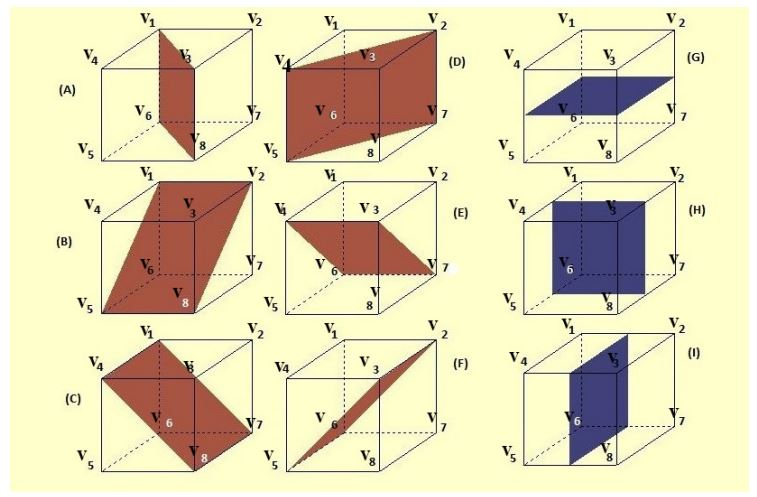
\includegraphics[width=16cm]{cube3.JPG}
\caption{Rotational Symmetry of a Cube}
\end{figure}\\
In short there are 24elements in a group of symmetry of a cube
\vspace{3cm}
\\
\subsection{SQUARE IN DIFFERENT DIMENSIONS}\\

\begin{enumerate}
    \item \textbf{Square in Dimension 4}: this is also called  tesseract. It is to a cube what a cube is to a square. Just as a cube is made up of square faces, a tesseract is made up of cube-like "cells." Each cell is a three-dimensional cube, and these cubes are connected in a way that forms a four-dimensional shape. It's important to note that we can't directly visualize a tesseract in our three-dimensional world.

    \item \textbf{Square in Dimension 5}: a square in five dimensions would be described as a five-dimensional polytope. In this case, it would be a polytope with five equal-length edges (sides) meeting at each vertex, and the angles between these edges would be right angles.
    \end{enumerate}
The following table and Figure 21 shows description of square in dimension four and five\\

\begin{tabular}{| l | l | l |l |l |}
\hline
Name& 	Dimensions& Number of edges& Number of vertices& No of Cubes\\
\hline
Tesseract& 	4& 	32& 16& 8\\
\hline
Five-cube& 	5& 	80& 32 & 40\\
\hline
\end{tabular}\\


\begin{figure}[htp]
     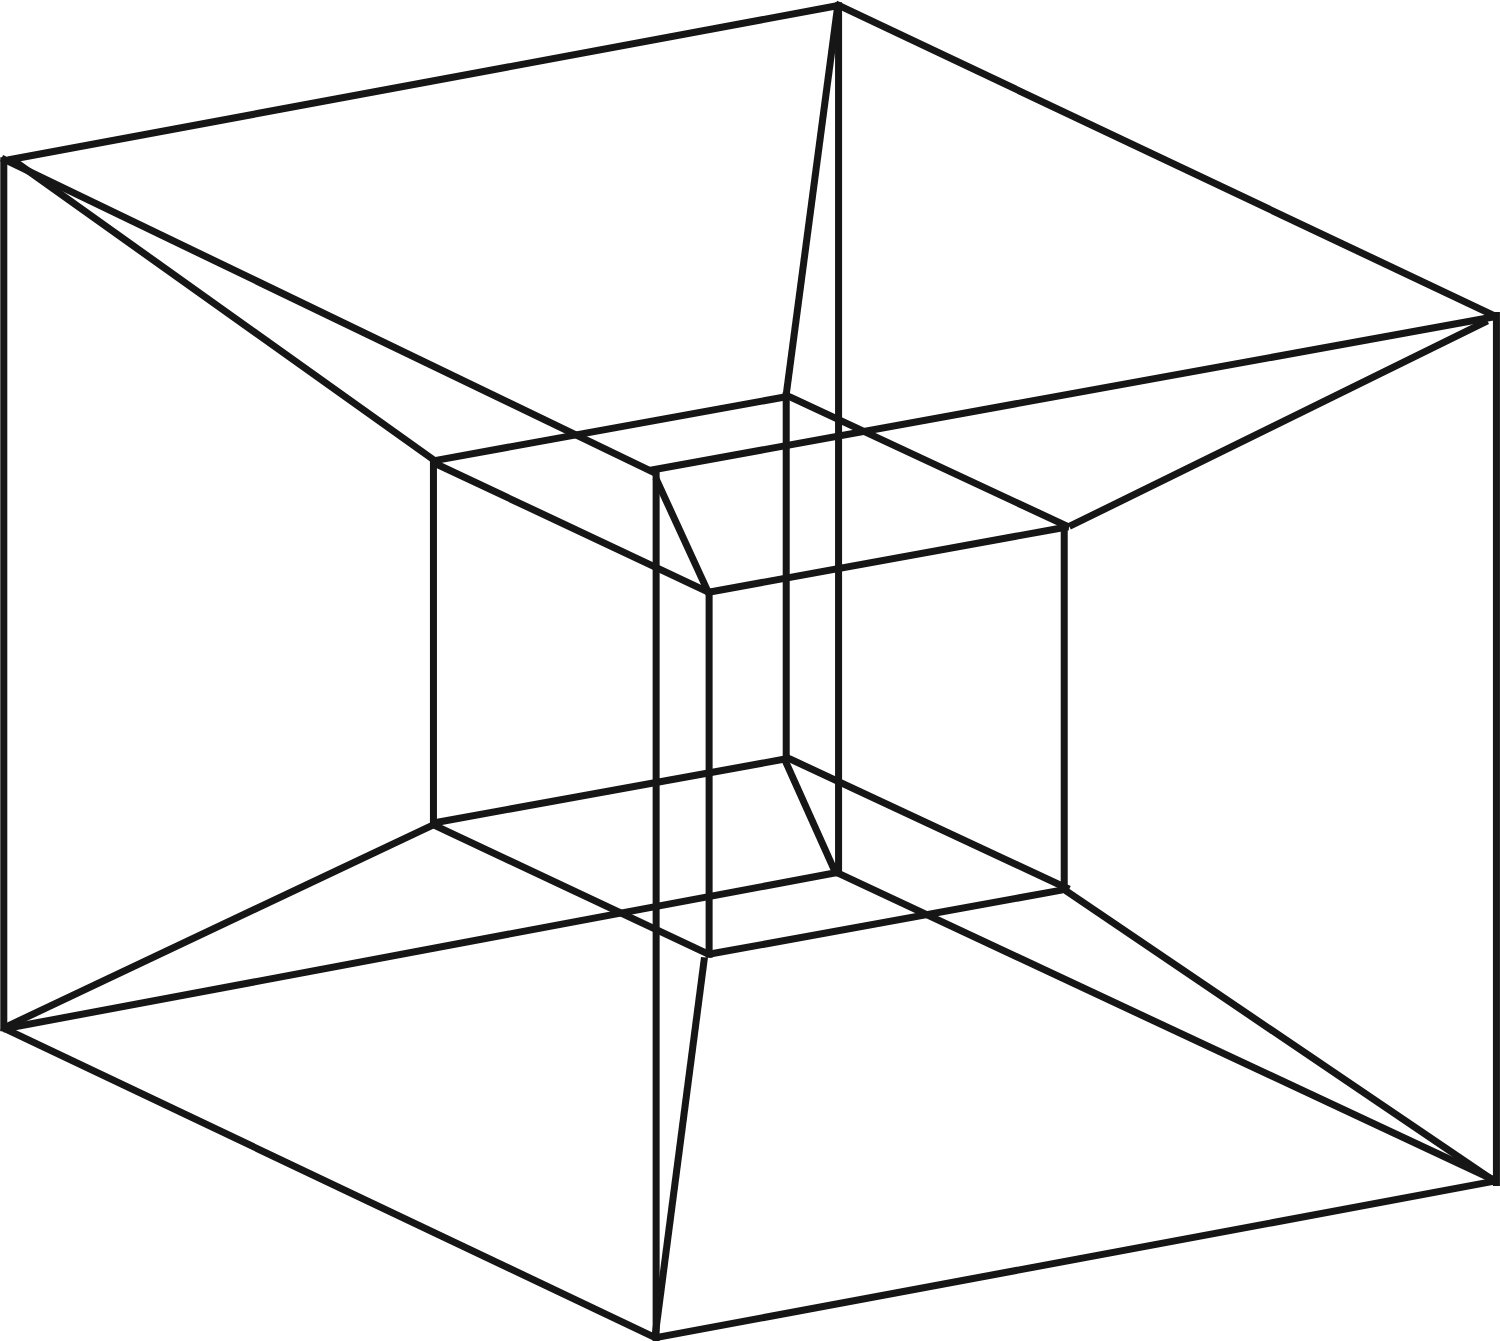
\includegraphics[width=7cm]{pictures/teresa.png}
     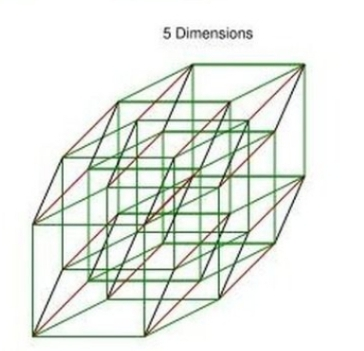
\includegraphics[width=7cm]{pictures/dimensionv.jpg}
     \caption{Tesseract and Five-cube}
\end{figure}
\vspace{9cm}
\section{PROJECT 4}
\pmb{Questions}\\
It holds true that any straight line passing through the origin within $\mathcal{R}^2$ forms a group in $\mathcal{R}^2$ with respect to addition. Can we extend this property to:
\begin{enumerate}
    \item Quadratic curves
    \item Cubic curves?
\end{enumerate}

Based on the information previously presented, which types of curves exhibit a group structure?\\\
\pmb{Solution}
\begin{enumerate}
    \item Quadratic Curves
Let A denotes the set of all quadratic curves passing through the origin defined by\\
$\mathcal{U}:=\{(x,y):y=ax^2+bx,$ $a,b,x,y \in \mathcal{R}, a \neq 0 \}$  \\
We shall show that $\mathcal{U}$ is not a group because it is not closed under addition.\\\\

\pmb{Proof}\\
Let $(x_1,y_1)$, $(x_2,y_2)$ such that $y_1=ax_1^2+bx_1$ and $y_2=ax_2^2+bx_2$ be two elements in $\mathcal{U}$ 
then,\\

$y_1+y_2=ax_1^2+bx_1+ax_2^2+bx_2=a(x_1^2+x_2^2)+b(x_1+x_2)$ ....(eqI)\\\\
Now let us add the two elements in $\mathcal{U}$ to see if it is closed or not\\
$(x_1,y_1)+(x_2,y_2) =(x_1+x_2,y_1+y_2)$
Assume $\mathcal{U}$ is closed then, 
$(x_1+x_2,y_1+y_2)$ will be an element in $\mathcal{U}$\\
that is, $(y_1+y_2)=a(x_1+x_2)^2+b(x_1+x_2)$ \\
But we aready see in eq I that $ y_1+y_2=a(x_1^2+x_2^2)+b(x_1+x_2)$\\
Since $a(x_1^2+x_2^2)+b(x_1+x_2) \neq a(x_1+x_2)^2+b(x_1+x_2)$ Therefore there is contradiction. \pmb{Hence, It is not closed}.

   \item Cubic Curves
Let $\mathcal{C}$ denotes the set of all quadratic curves passing through the origin defined by\\
$\mathcal{C}:=\{(x,y):y=ax^3+bx^2+cx,$ $a,b,c,x,y \in \mathcal{R}, a \neq 0 \}$  \\
We shall show that $\mathcal{C}$ is not a group because it is not closed under addition.\\\\

\pmb{Proof}\\
Let $(x_1,y_1)$, $(x_2,y_2)$ such that $y_1=ax_1^3+bx_1^2+cx_1$ and $y_2=ax_2^3+bx_2^2+cx_2$ be two elements in $\mathcal{C}$ 
then,\\
$y_1+y_2=ax_1^3+bx_1^3+cx_1+ax_2^3+bx_2^2+cx_2=a(x_1^3+x_2^3)+b(x_1+x_2^2)+c(x_1+x_2)$ ....(eqI)\\\\
Now let us add the two elements in $\mathcal{C}$ to see if it is closed or not\\
$(x_1,y_1)+(x_2,y_2) =(x_1+x_2,y_1+y_2)$\\
Assume $\mathcal{C}$ is closed then, 
$(x_1+x_2,y_1+y_2)$ will be an element in $\mathcal{C}$\\
that is, $(y_1+y_2)=a(x_1+x_2)^3+b(x_1+x_2)^2+c(x_1+x_2)$ \\
But we already see in eq I that $ (y_1+y_2)=a(x_1^3+x_2^2)+b(x_1+x_2)^2+c(x_1+x_2)$\\
Since $a(x_1^3+x_2^3)+b(x_1^2+x_2^2)+c(x_1+x_2) \neq a(x_1+x_2)^3+b(x_1+x_2)^2+c(x_1+x_2)$\\
Therefore there is contradiction. \pmb{Hence, It is not closed.}






\end{enumerate} 


\end{document}
